% -*- mode: noweb; noweb-default-code-mode: R-mode; -*-
%\VignetteIndexEntry{Using Director}
\documentclass[a4paper]{article}

\title{Director}
\author{Katherine Icay}


\usepackage{a4wide}
\usepackage{ragged2e}
\usepackage{hyperref}
\usepackage{dirtree}

\usepackage{Sweave}
\begin{document}
\Sconcordance{concordance:vignette.tex:vignette.Rnw:%
1 13 1 1 0 71 1 1 2 1 0 1 8 10 0 1 3 18 0 1 2 1 1 1 8 7 0 1 4 6 0 1 3 %
18 0 1 2 30 1 1 2 1 0 2 1 3 0 1 2 5 1 1 2 1 0 2 1 3 0 1 2 10 1 1 4 4 0 %
1 3 18 0 1 2 17 1 1 4 3 0 1 4 2 0 1 5 6 0 1 2 33 1}

\newenvironment{blockquote}{%
    \par%
    \medskip
    \leftskip=4em\rightskip=2em%
\ignorespaces\justify}{%
    \par\medskip}
\maketitle

\begin{blockquote}
\begin{center}\textbf{Abstract}\end{center}
\noindent \textit{Director} is an R package designed to streamline the visualization of multiple levels of interacting RNA-seq data.  It utilizes a modified Sankey plugin of the JavaScript library D3 to provide a fast and easy, web-based solution to discovering potentially interesting downstream effects of regulatory and/or co-expressed molecules. The diagrams are dynamic, interactive, and packaged as HTML files -- making them highly portable and eliminating the need for third-party software. This enables a straightforward approach for scientists to interpret the data produced, and bioinformatics developers an alternative means to present relevant data.
\end{blockquote}

\tableofcontents

\section{Sankey diagram}
    \subsection{What is it?}
Sankey diagrams are types of flow diagrams comprised of paths and nodes designed to represent flow measurements within a system of distinct events. They are particularly useful for identifying the contributions of these events in a directional cascade, with larger downstream contributions emphasized by making path widths proportional to input values. This package takes advantage of this feature to visualize multiple levels of interacting molecules in a directional flow; offering novel presentation of key findings from complex datasets and dynamic, visual analysis of downstream regulatory effects. 

Dynamic visualization of data is achieved with the Sankey plugin of Mike Bostock's JavaScript library, \href{http://d3js.org/}{D3}. Compared to traditional Sankey diagrams, this package provides novel drawing capabilities to better depict molecular interactions. By enabling input for both path and node values, colours are meaningfully assigned according to a gradient scale rather than being assigned randomly or uniformly. Furthermore, in molecular biology, both positive and negative measurement values are of interest and thus both extremes are scaled for when drawing path widths.

    \subsection{Limitations}
Sankey diagrams are strictly directional flow diagrams and are not suitable for depicting feedback loops (i.e. a path from one node that leads back to itself). Order of input is also important: \textit{all} upstream connections must precede downstream connections to successfully draw the diagram. For example, a list must contain all miRNA-mRNA pairs first, mRNA-gene pairs second.

As with all data-driven diagrams, large datasets can be difficult or impossible to visualize and still be able to distinguish individual nodes and paths. While this package does not restrict the amount of paths and nodes defined, it will warn users that the diagram may not be rendered correctly. In most cases, this means less connected paths and nodes may be too small to be rendered at all. In this situation, users have two options: (1) filter the data manually or using the quantitative and qualitative filters of the package, and/or (2) manually define the diagram height and width to be large enough to render all nodes and paths. Instructions on how to perform these actions are described below. 

    \subsection{Diagram features}
One advantage of an HTML output is that it encourages user interaction with the data. Quantitative and qualitative information about each node and path are easily referenced with mouseover. Nodes are dynamic and can be moved around the space for optimal presentation. Furthermore, entire pathways can be highlighted in the overall diagram by clicking on the node (or nodes) of interest.

\begin{figure}[htbp]
    \begin{center}
    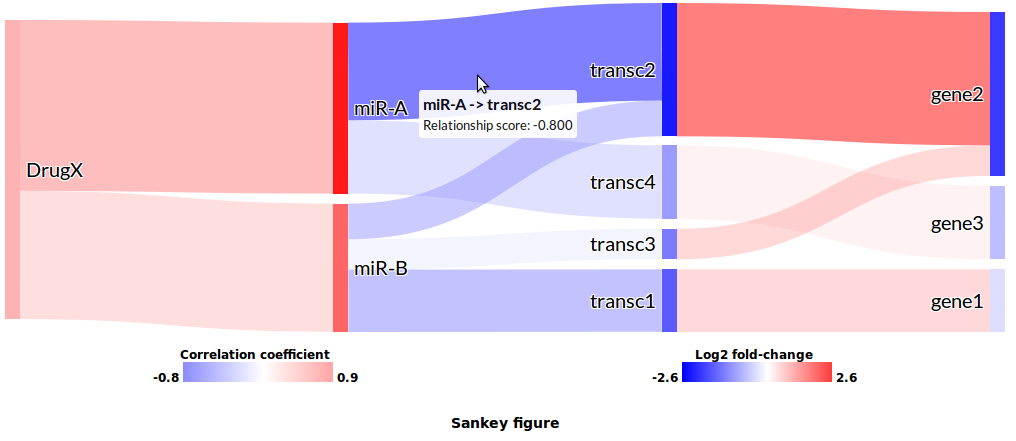
\includegraphics[width=\textwidth]{figure4.png}
        \caption{Sankey plot with mouseover information and connected paths to \textit{transc2} highlighted.}
    \end{center}
\end{figure}

\section{Standard workflow}
    \subsection{Getting started}
First, a working directory must be specified and initialized with $initSankey$. This writes the necessary scripts enabling dynamic HTML and specifies the basic look of the figures. Specifically, the D3 JavaScript library (currently, version 3.5.6) and Mike Bostock's D3 plugin for Sankey. The function requires no inputs but optional parameters can be used to define an absolute path (default is the working directory obtained from $getwd()$), alternate download links to necessary scripts and download methods, path opacity, font, and font sizes of node labels.

Running $initSankey$ in the working directory produces the following files and folders:
\dirtree{%
.1 /.
.2 css.
.3 sankey.css.
.2 js.
.3 d3.min.js.
.3 d3.v3.js.
.3 LICENSE.
.3 sankey.js.
.2 layouts.
.3 charts.html.
.2 config.yml.
}

These files are necessary for functions $makeSankey$ and $drawSankey$ to work so it must always be executed first. The parameters defined in $initSankey$ will apply to all HTML files written to the specified directory. Rerunning this function with different parameters will, therefore, alter the look of all HTML files within the directory (see section~\ref{sec:figMods} and Figure~\ref{fig:Custom}).

    \subsection{Input data}
\textit{Director} requires two types of quantitive information as input: values for \textit{nodes} and values for \textit{paths}. The package assumes nodes are molecules of interest and that the quantitative value is the feature which makes them interesting, e.g. expression fold-change, significance value, or methylation score. Similarly, paths represent a predictive or quantitative measure of the interaction between molecules (e.g. correlation, affinity score).

Node and path values can be input in two ways.
    \begin{enumerate}
        \item As a single table with each row defining a source node, target node, relationship value, node values, and (optional) descriptive information.
        \item As two separate tables: one with each row defining a source node, target node, relationship value, and (optional) descriptive values; and another with two columns defining all nodes and corresponding node values.
    \end{enumerate}

\noindent Suppose we have the following information:\\
\begin{center}
    \begin{tabular}{lllll} \hline
    source & target & impact score & source fold-change & target fold-change\\ \hline
    DrugX & miR-B & 0.6 & 1 & 1.5\\
    DrugX & miR-A & 0.8 & 1 & 2.6\\
    miR-B & transc1 & -0.7 & 1.5 & -1.7\\
    miR-B & transc2 & -0.4 & 1.5 & -2.6\\
    miR-B & transc3 & -0.34 & 1.5 & -1.5\\
    miR-A & transc2 & -0.8 & 2.6 & -2.6\\
    miR-A & transc4 & -0.6 & 2.6 & -1.2\\
    trasc1 & gene1 & 0.8 & -1.7 & -0.6\\
    transc2 & gene2 & 0.9 & -2.6 & -2.2\\
    transc3 & gene2 & 0.88 & -1.5 & -2.2\\
    transc4 & gene3 & 0.6 & -1.2 & -0.7\\ \hline
    \end{tabular}\\
\end{center}

\noindent We define information for a Sankey diagram with the function $createList$ which takes as input either a single table:
\begin{Schunk}
\begin{Sinput}
> library(Director)
> table1 <- data.frame(source=c("DrugX", "DrugX", "miR-B", "miR-B", "miR-B",
+         "miR-A", "miR-A", "transc1", "transc2", "transc3", "transc4"),
+     target=c("miR-B", "miR-A", "transc1", "transc2", "transc3", "transc2",
+         "transc4", "gene1", "gene2", "gene2", "gene3"),
+     value=c(0.6, 0.8, -0.7, -0.4, -0.34, -0.8, -0.6, 0.8, 0.9, 0.88, 0.6),
+     sourcefc=c(1,1,1.5,1.5,1.5, 2.6,2.6,-1.7,-2.6,-1.5,-1.2),
+     targetfc=c(1.5,2.6,-1.7,-2.6,-1.5,-2.6,-1.2,-0.6,-2.2,-2.2,-0.7),
+     stringsAsFactors=FALSE)
\end{Sinput}
\end{Schunk}
\begin{Schunk}
\begin{Sinput}
> tempList <- createList(table1)
\end{Sinput}
\begin{Soutput}
    source  target description value sourcefc targetfc
1    DrugX   miR-B              0.60      1.0      1.5
2    DrugX   miR-A              0.80      1.0      2.6
3    miR-B transc1             -0.70      1.5     -1.7
4    miR-B transc2             -0.40      1.5     -2.6
5    miR-B transc3             -0.34      1.5     -1.5
6    miR-A transc2             -0.80      2.6     -2.6
7    miR-A transc4             -0.60      2.6     -1.2
8  transc1   gene1              0.80     -1.7     -0.6
9  transc2   gene2              0.90     -2.6     -2.2
10 transc3   gene2              0.88     -1.5     -2.2
11 transc4   gene3              0.60     -1.2     -0.7
\end{Soutput}
\end{Schunk}

\noindent Or two separate tables:
\begin{Schunk}
\begin{Sinput}
> List <- data.frame(source=c("DrugX", "DrugX",
+         "miR-B", "miR-B", "miR-B", "miR-A", "miR-A", "transc1",
+         "transc2", "transc3", "transc4"),
+     target=c("miR-B", "miR-A", "transc1", "transc2", "transc3",
+         "transc2", "transc4", "gene1", "gene2", "gene2", "gene3"),
+     value=c(0.6, 0.8, -0.7, -0.4, -0.34, -0.8, -0.6, 0.8, 0.9, 0.88, 0.6),
+     	    stringsAsFactors=FALSE)
> ListFC <- data.frame(genes=c("DrugX", "miR-B", "miR-A", "transc1",
+     "transc2", "transc3", "transc4", "gene1", "gene2", "gene3"),
+     foldChange=c(1, 1.5, 2.6, -1.7, -2.6, -1.5, -1.2, -0.6, -2.2, -0.7),
+         stringsAsFactors=FALSE)
\end{Sinput}
\end{Schunk}
\begin{Schunk}
\begin{Sinput}
> tempList2 <- createList(List,ListFC)
\end{Sinput}
\begin{Soutput}
    source  target description value sourcefc targetfc
1    DrugX   miR-B              0.60      1.0      1.5
2    DrugX   miR-A              0.80      1.0      2.6
3    miR-B transc1             -0.70      1.5     -1.7
4    miR-B transc2             -0.40      1.5     -2.6
5    miR-B transc3             -0.34      1.5     -1.5
6    miR-A transc2             -0.80      2.6     -2.6
7    miR-A transc4             -0.60      2.6     -1.2
8  transc1   gene1              0.80     -1.7     -0.6
9  transc2   gene2              0.90     -2.6     -2.2
10 transc3   gene2              0.88     -1.5     -2.2
11 transc4   gene3              0.60     -1.2     -0.7
\end{Soutput}
\end{Schunk}

\noindent Note that \textit{description} is a required column to make and draw a Sankey diagram. If it is not defined in $createList$, an empty \textit{description} column will be created. This column can be used, for example, to provide the gene name of a target transcript or additional information about the source and target interaction. Descriptive information can be written in HTML code and are accessed via mouseover of the respective paths.

\section{Data filtering}
\textit{Director} has several functions that attempt to streamline the visualization process. For useful and efficient visualization, data should first be filtered for the most valuable, user-defined set of information.

\subsection{What's being visualized?}
Hundreds and thousands of molecules can be detected in a single living cell at any given time. Molecules that have mRNA content sequenced and quantified are considered 'expressed', but are not necessarily interesting. In fact, depending on the questions a user wishes to answer, most of the expressed molecules are noise and the potentially interesting molecules difficult to distinguish.

Basic functions are provided with \textit{Director} to filter the list of source and target nodes for:
\begin{itemize}
    \item $filterNumeric$ Minimum, maximum, or absolute numerical values.
    \item $filterSubset$ User-defined qualitative values grep'd from up to two qualitative columns (e.g. source and target).
    \item $filterRelation$ Positively correlated or inversely related source-target pair node or path values.
\end{itemize}
\noindent Multiple lists can be created representing different levels of source-target relationships and combined with $append2List$. The package then visually organizes downstream effects to several biologically functional levels. See the package manual for more details and examples for each function.

\section{Visual parameters}
After filtering, the ready list is input to $makeSankey$. This function calculates and assigns drawing values for nodes, assigns colours to nodes, and assigns colours to paths. A red-blue palette is used by default to render diagrams, but colour ranges for both nodes and paths can be defined separately. $drawSankey$ then takes these values to create the HTML containing the interactive Sankey diagram. These HTML files can then be saved to the working directory with $writeSankey$, where the supporting files generated with $initSankey$ are already saved.

\subsection{Nodes and paths}
The primary function of the package is to render a custom Sankey diagram with paths and nodes assigned colours based on quantitative measures.

\begin{figure}[htbp]
    \begin{center}
    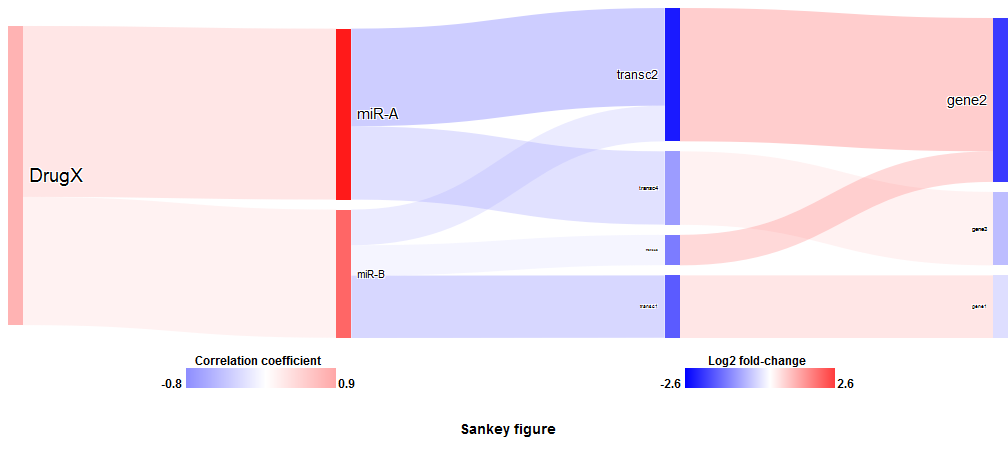
\includegraphics[width=\textwidth]{figure1.png}
    \caption{Sankey plot}
    \end{center}
\end{figure}

Before drawing the diagram, colour scales  must first be assigned to the node and path values.
\begin{Schunk}
\begin{Sinput}
> initSankey()
> sankey <- makeSankey(tempList2)
> drawSankey(sankey)
\end{Sinput}
\end{Schunk}

By default, this package assumes larger absolute values are stronger than smaller values. However, some values (e.g. significance levels)  are stronger with smaller values and weaker with larger ones. In these cases, \textit{nought} or zero values can be defined for either paths or nodes such that stronger colors are given to smaller values and weaker colors to larger values. This makes the diagram robust to a wide range of data input and able to match almost any colour theme. Furthermore, both names and hexidecimal codes can be input as colour values.

    \subsubsection{\textit{averagePath} parameter}
What if there is no unique path values after the first level of interacting nodes? What if interest is only in the downstream effect of the first level of interactions (e.g. drugs and their molecular targets)? $makeSankey$ has a Boolean parameter called \textit{averagePath} that, when set to $TRUE$, will replace the \textit{List\$value} of a source-target pair of molecules (say, miRNA-1 and target Gene A) with an average value of the incoming paths to the source molecule (say, Drug X and Drug Y targeting miRNA-1). Assuming a uniform downstream effect, this colours downstream paths in the figure based on the average effect of the initial level of source-target values. Consequently, this gives more emphasis to the quantitative node values.

\begin{Schunk}
\begin{Sinput}
> initSankey()
> sankey2 <- makeSankey(tempList2, averagePath=TRUE)
> drawSankey(sankey2)
\end{Sinput}
\end{Schunk}

\begin{figure}[htbp]
    \begin{center}
    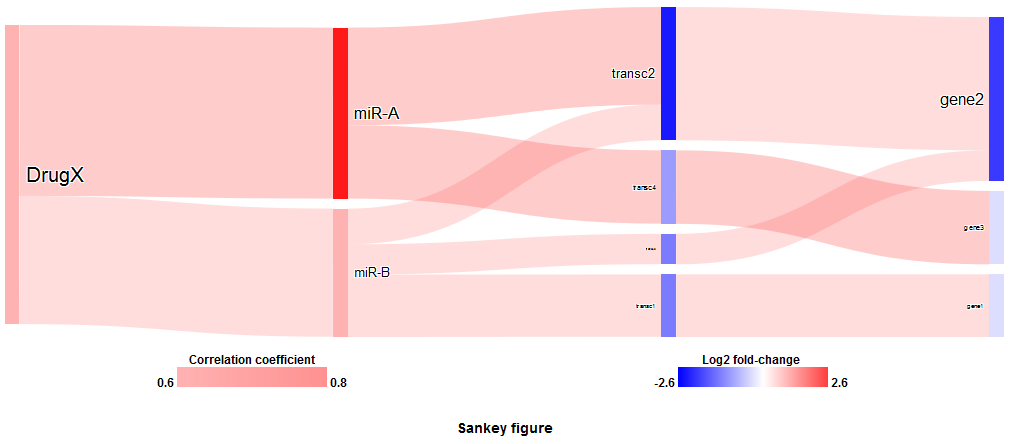
\includegraphics[width=\textwidth]{figure2.png}
    \caption{Sankey plot with averagePath enabled.}
    \end{center}
\end{figure}

Note the value differences with and without averagePath enabled.

\begin{Schunk}
\begin{Sinput}
> truevalue <-  sankey$reference[,"truevalue"]
\end{Sinput}
\end{Schunk}
\begin{Schunk}
\begin{Sinput}
> cbind(sankey2$reference[,c("source", "target","averagePath_value")],truevalue)
\end{Sinput}
\begin{Soutput}
    source  target averagePath_value truevalue
1    DrugX   miR-B               0.6      0.60
2    DrugX   miR-A               0.8      0.80
3    miR-B transc1               0.6     -0.70
4    miR-B transc2               0.6     -0.40
5    miR-B transc3               0.6     -0.34
6    miR-A transc2               0.8     -0.80
7    miR-A transc4               0.8     -0.60
8  transc1   gene1               0.6      0.80
9  transc2   gene2               0.7      0.90
10 transc3   gene2               0.6      0.88
11 transc4   gene3               0.8      0.60
\end{Soutput}
\end{Schunk}

    \subsection{Figure dimensions and properties}
Each figure includes a legend containing the colour scales for node values and for path values. $drawSankey$ parameters allow customization of the legend font, font size, legend content, and figure caption.

By default, figures are drawn with a 1000px width and height adjusted to the number of nodes/unique molecules up to 1800px (or approximately 300 nodes). If the figure fails to appear in the HTML file with $drawSankey$ defaults, the options are either to
\begin{enumerate}
    \item Define $drawSankey$ parameters \textit{height} > 1800px and \textit{width} > 1000px.
    \item Use \textit{Director} filters to reduce the number of nodes to draw.
\end{enumerate}

The goal of this package is to highlight key molecules and regulatory interactions. Having more molecules than necessary makes the figure 'noisy'.

Fortunately, users can view quantitative and qualitative information, including optional descriptions, directly from nodes and paths in the diagram via mouseover. This is useful to determine, for example, what quantitative thresholds to filter for to remove uninteresting paths from the figure.

    \subsubsection{Figure modifications}
    \label{sec:figMods}
When any part of the List information is modified, $makeSankey$ needs to be rerun to update colour assignments (quantitative values), nodes, and path connections. Changes to the general appearance of the figure can be made with parameters in $initSankey$ and $drawSankey$. Details are available in the manual. To update the figure with the changes, simply rerun $drawSankey$. Figure 4 is drawn with the exact same List information as Figure 3 but using non-default parameters.

\begin{Schunk}
\begin{Sinput}
> initSankey(pathOpacity = 0.3, pathHover = 0.6,
+     fontsizeProportion = FALSE, fontsize=20)
> # Makes the path colours darker by 10%  and uses a single, uniform font size
> # for the figure rather than font sizes proportional to node size.
> 
> sankey2 <- makeSankey(tempList2, averagePath=TRUE,
+     nodeMin = "orange", nodeMax = "purple", pathMax = "#333333")
> # Changes the default colours used.
> 
\end{Sinput}
\end{Schunk}
\begin{Schunk}
\begin{Sinput}
> drawSankey(sankey2, caption = "Alternate figure",
+     nodeValue = "Node colour scale", pathValue = "Path colour scale",
+     legendsize = 14, height = 300)
> # Changes to legend values and overall figure size
\end{Sinput}
\end{Schunk}

\begin{figure}[htbp]
    \begin{center}
    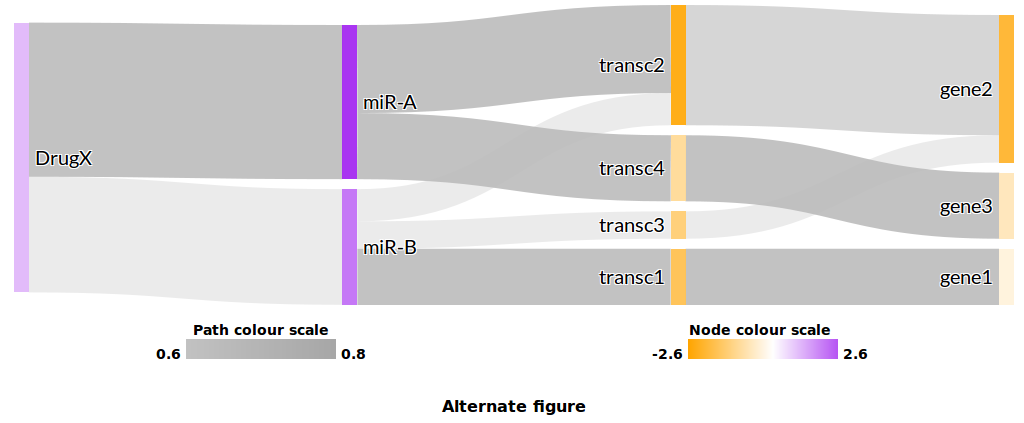
\includegraphics[width=\textwidth]{figure3.png}
    \caption{Sankey plot with averagePath enabled and non-default parameters.}
    \label{fig:Custom}
    \end{center}
\end{figure}

\section{Saving data}
The relevant outputs generated are:
\begin{enumerate}
    \item The List created with $createList$ used as input for the main Sankey functions.
    \item The Sankey diagram produced with $drawSankey$.
\end{enumerate}
The former is a standard R data frame and can be saved with normal methods, e.g. $write.table()$. This simplifies later usage as it is already in the appropriate List format and can immediately be used with filtering and Sankey functions.

The latter can be saved to file using the function $writeSankey$. HTML has the dual benefit of preserving information dynamics of the diagram and vector graphics quality. As a result, adjusting the flow of the diagram and saving as a high-quality PDF (or .png) in any dimension is simple.


\end{document}
